\documentclass[11pt]{article}
\usepackage[T1]{fontenc}
\usepackage{lmodern,microtype,amsmath,amssymb,amsthm,mathtools,booktabs,array,xurl}
\usepackage[a4paper,margin=28mm]{geometry}
\usepackage{tikz}
\usetikzlibrary{arrows.meta,positioning,calc}
\usepackage[colorlinks=true,linkcolor=blue!55!black,citecolor=blue!55!black,urlcolor=blue!55!black]{hyperref}
\setlength{\emergencystretch}{2em}
\numberwithin{equation}{section}
\newtheorem{theorem}{Theorem}[section]
\newtheorem{proposition}[theorem]{Proposition}
\newtheorem{lemma}[theorem]{Lemma}
\newtheorem{corollary}[theorem]{Corollary}
\theoremstyle{definition}\newtheorem{definition}[theorem]{Definition}
\theoremstyle{remark}\newtheorem{remark}[theorem]{Remark}
\newcommand{\ii}{\mathrm i}
\newcommand{\dd}{\mathrm d}
\newcommand{\Vol}{\operatorname{Vol}}
\newcommand{\Ch}{\operatorname{Ch}}
\newcommand{\Turn}{\mathsf T}
\newcommand{\stat}{\operatorname{stat}}
\newcommand{\Log}{\operatorname{Log}}
\title{Local degree and twist bounds for circle-tree volume limits}
\author{}\date{}
\begin{document}\maketitle
\begin{abstract}
We prove a volume limit for the original reduced invariant of a fixed
ordered tree of crossing circles from a finite condition at its vertices.
The condition allows a different real-decay bound on each directed edge
and imposes no sum over the tree. A simple consequence is that at every
vertex either the degree is at least \(2^{28}\) or the absolute signed
crossing power is at least \(2^{27}\). Large-degree vertices may retain
zero or small powers. The proof evaluates the full finite contraction
recursively, dividing each subtree polynomial by its exact value at zero.
A conditional complex kernel estimate, a one-variable Fourier calculation
with all endpoint currents, and a fresh outgoing bound close the induction
without a depth-dependent exponential loss. The leading coefficient is
nonzero through both level parities. The classical circle-tree theorem
identifies the critical action with the volume of the original hyperbolic
knot complement. We retain the microscopic main-meridian scalar and give
its normalized leading profile.
\end{abstract}

\section{The fixed diagrams and the conclusion}\label{dt:intro}
A crossing circle bounds a disk punctured twice by the main strands.
Its signed crossing power is measured in that disk's original frame.
Fix a finite ordered tree \(\mathcal T=(V,E)\), with at least one edge,
and a crossing-circle tangle \(P_v\) at every vertex. The literal rooted
construction is
\[
 W_v=\left(\prod_{w\in I_v^-}\Turn(W_w)\right)P_v
           \left(\prod_{w\in I_v^+}\Turn(W_w)\right).
\]
The lists have their specified orders. Each turn rotates the whole tangle
and its disk frame. There are no bare product junctions. Draw the
prescribed terminal-root cylindrical closure with its actual strand
orientations and one reduced cut on a main strand. Require that endpoint
tracing gives one main component and no component already closed inside
an intermediate tangle. These are the diagram hypotheses of
\cite[Section~1]{Geometry}; the abstract tree alone does not imply them.

Write \(d_v\ge1\) for the graph degree and \(n_v\in\mathbb Z\) for the
physical signed crossing power. The diagram and every power are fixed
before the integer level \(N\ge3\) tends to infinity. Put
\[
 q_N=e^{\pi\ii/N},\qquad d=N-1,\qquad M=q_N^s,\qquad |s|\le R<1.
\]
The level degree \(d\) is distinct from \(d_v\). Let \(F_N(M)\) be the
reduced zero-framed ADO invariant in the convention of \cite{Meridian},
with unknot value one. At \(M=1\) it is the reduced Kashaev invariant of
the same knot \(K_{\mathbf n}\). The cut, orientation and framing are
retained in every finite contraction below.

Choose any vertex \(o\) as the final vertex for evaluating that
contraction. Section~\ref{dt:criterion} gives a finite criterion in
\(d_v,n_v,o\) and numbers \(0<c_v<2^{-16}\) attached to the nonroot
vertices. The number \(c_v\) is a chosen bound for the normalized
polynomial sent from \(v\) to its parent. Its definition uses no unknown
invariant or critical value.

For the action, let
\[
 J(x)=\int_0^x\log(2\sin\pi u)\,\dd u,\qquad
 g(x)=J(2x)-4J(x),\qquad G_0=g(1/4).
\]
The even holomorphic edge phase near \((0,0)\) is specified by
\begin{equation}\label{dt:psi}
 \psi(0,0)=2G_0,\qquad
 \psi_t(t,u)=-\frac1\pi\operatorname{arsinh}
                       \bigl(\tan(t/2)\cos(u/2)\bigr),
 \qquad\psi_u(t,u)=\psi_t(u,t).
\end{equation}
Branches continue from zero; the mixed derivatives agree. Put
\[
 \Psi(\boldsymbol\tau)=\sum_{vw\in E}\psi(\tau_v,\tau_w),\qquad
 \mathcal C=\operatorname{stat}_{\boldsymbol\tau}
 \left\{\Psi(\boldsymbol\tau)+\frac{\ii}{4\pi}
             \sum_v n_v\tau_v^2-\ii\sum_v\tau_v\right\}.
\]
The proof constructs the small critical point used in this notation.

\begin{theorem}\label{dt:main}
Suppose the chosen root and bounds \(c_v\) satisfy the directed criterion
\eqref{dt:eq-3}, \eqref{dt:eq-8}, \eqref{dt:eq-9}.
There is a constant \(D_{\mathcal T,\mathbf n}\ne0\), independent of
level parity, such that
\begin{equation}\label{dt:leading}
 F_N(1)=\Omega_N N^{3/2}D_{\mathcal T,\mathbf n}
                  e^{N\mathcal C}(1+O(N^{-1})),\qquad
 \Omega_N=q_N^{d^2(2w(D)+\sum_vn_v)/4}.
\end{equation}
Here \(w(D)\) is the original oriented writhe and \(|\Omega_N|=1\).
The original knot complement is hyperbolic, and
\begin{equation}\label{dt:volume}
 \lim_{N\to\infty}\frac{2\pi}{N}\log|F_N(1)|
       =2\pi\Re\mathcal C=\Vol(S^3\setminus K_{\mathbf n}).
\end{equation}
Moreover, with
\begin{equation}\label{dt:scalars}
 H_N(s)=\frac{\sin\pi s}{N\sin(\pi s/N)},\qquad
 A_N(s)=q_N^{(-w(D)-\sum_vn_v)s^2/2},
\end{equation}
where \(H_N(0)=1\), one has uniformly for \(|s|\le R<1\)
\begin{equation}\label{dt:profile}
 \frac{F_N(q_N^s)}{A_N(s)H_N(s)F_N(1)}=1+O_R(N^{-1}).
\end{equation}
These values are nonzero for all sufficiently large \(N\), and the volume
limit holds uniformly with \(F_N(q_N^s)\) in place of \(F_N(1)\).
\end{theorem}
All implied constants and starting levels may depend on the fixed tree,
its powers and \(R\). The numerical curvature bounds and the directed
criterion do not acquire an extra constant from the depth of the tree.

\begin{corollary}\label{dt:mixed}
The theorem holds if, independently at each vertex,
\[
 \boxed{\quad d_v\ge2^{28}\quad\hbox{or}\quad |n_v|\ge2^{27}.\quad}
\]
It also holds under the uniform local condition
\(\max_v d_v/(d_v^2+n_v^2)\le2^{-120}\).
\end{corollary}
The proof of the corollary is in Section~\ref{dt:sec-8}; it covers all
degrees symbolically. The tree, its degrees and all powers remain fixed.
A high-degree vertex may have \(n_v=0\). Neither condition is a
hypothesis that the sum of \(d_v/(d_v^2+n_v^2)\) is small.

\paragraph{Inputs and proof boundary.}
The exact finite inputs are \cite[Proposition~6.1, Theorem~7.1 and
Proposition~8.1]{Meridian}: full crossing polynomials and traces, original
typed tree contraction, and scalar ledger. The unconditional estimates
in \cite[Lemma~2.1, Sections~3--4 and Section~6.1]{Summed} supply
polynomial norm comparisons, the complex edge sum and the exact
one-variable Fourier conversion. Their proofs use no summed criterion.
Canonical factorial interpolation is \cite[Lemma~2.1]{Factorial}.
The geometric input is \cite[Theorem~1.1]{Geometry}, whose degree-and-twist
threshold follows from our criterion. We prove the conditional
normalization, directed bounds, complete recursive induction and
noncancellation here. No all-orders expansion, longitude factor, larger
strict Conway grammar or fixed \(M\)-neighborhood is asserted.

\section{A finite criterion on directed edges}\label{dt:criterion}
The root in this section is an order for evaluating the closed finite
contraction. It need not be the terminal root used to draw the original
knot. A nonroot vertex sends one polynomial to its parent; the last
vertex sends none. The following constants and inequalities reflect
that difference.

Put

\begin{equation}\label{dt:eq-1}
\begin{gathered}
a_0=\frac1{2\pi},\qquad k_0=2^{-16},\qquad
 R_0=\frac18,\qquad b_0=2^{-11},\qquad\\
 r_0=\frac1{16},\qquad t_0=2^{-14},\qquad
 \chi=1-\cos r_0.
\end{gathered}
\end{equation}

The parent-variable rectangle is

\begin{equation}\label{dt:eq-2}
\mathcal R=\{u:|\Re u|\le R_0,\ |\Im u|\le b_0\}.
\end{equation}

Choose any vertex as root and direct all edges toward it. For every
nonroot vertex choose a number

\begin{equation}\label{dt:eq-3}
0<c_v<k_0,
 \qquad
 \delta_v=\min\left\{\frac{b_0}2,
               \frac{c_v\chi}{4(1+c_v)}\right\}.
\end{equation}

These are parameters of the criterion. They can differ at every edge.
They are not asymptotic quantities to be inferred from the invariant.

Write \(q_v=1\) at a nonroot vertex and \(q_v=0\) at the root. If \(\mathrm{Ch}(v)\) is the
set of children, define

\begin{equation}\label{dt:eq-4}
\begin{aligned}
 a_v&=\frac{d_v}{2\pi},& b_v&=\frac{n_v}{2\pi},&
 D_v&=a_v-i b_v,\\
 A_v&=\frac2{\pi^2}
       \left(q_vk_0+\frac12\sum_{w\in\mathrm{Ch}(v)}c_w\right),&
 B_v&=16q_v+|\mathrm{Ch}(v)|,&
 C_v&=B_v+\frac{b_v^2}{4A_v}.
\end{aligned}
\end{equation}

There is at least one incidence at every vertex, so \(A_v,B_v\) are positive.
Let

\begin{equation}\label{dt:eq-5}
\delta_v^{\mathrm{in}}
      =\min\bigl(\{b_0\}\cup
                     \{\delta_w:w\in\mathrm{Ch}(v)\}\bigr)
\end{equation}

and set

\begin{equation}\label{dt:eq-6}
y_v=\min\left\{
 \frac{\delta_v^{\mathrm{in}}}2,
 \frac{t_0|D_v|}{4C_v},
 \frac{A_v\pi^2}{8(\pi|b_v|+t_0|D_v|)},
 \sqrt{\frac{A_v\pi^2}{8B_v}}
 \right\}.
\end{equation}

Finally define two action quantities

\begin{equation}\label{dt:eq-7}
\beta_v=\frac{210}{361}\frac{a_v}{|D_v|^2},
 \qquad
 \eta_v=\min\left\{
 \frac12t_0|D_v|y_v,
 \frac12A_v\pi^2,
 A_vr_0^2,
 \frac18a_vr_0^2
 \right\}.
\end{equation}

The criterion consists of the strict inequalities

\begin{equation}\label{dt:eq-8}
\boxed{\quad t_0|D_v|\ge2,\qquad
                 \beta_v<\frac{\eta_v}{2}\quad
                      \text{at every vertex},\quad}
\end{equation}

and, only at nonroot vertices,

\begin{equation}\label{dt:eq-9}
\boxed{\qquad
       \beta_v<(k_0-c_v)\chi.\qquad}
\end{equation}

It is a finite elementary test in the degrees, signed powers, root and
positive numbers \(c_v\). It uses no value of an unknown quantum invariant
and no assumed dominance of a global saddle. Its quantities are local:
\(A_v\) and the available strip depend on the child budgets, while the exact
child scalar will be divided out rather than estimated.


We say that the chosen root and numbers \(c_v\) satisfy the directed
criterion when \eqref{dt:eq-3}, \eqref{dt:eq-8} and \eqref{dt:eq-9} hold.
No numerical estimate of an invariant enters this definition.
The number \(\beta_v\) bounds the action lost in evaluating just the
current trace after exact child constants are divided out. The four
entries of \(\eta_v\) pay, respectively, for the infinite charge tail,
the original endpoints, localization to a real interval, and its
vertical connecting paths. The extra comparison \eqref{dt:eq-9} is used
only to produce an outgoing real bound.

\section{The full kernel with a fixed parent angle}\label{dt:sec-2}

The fixed Newton polynomials are

\begin{equation}\label{dt:eq-N1}
\begin{gathered}
 d=N-1,\qquad c_j=2\cos((2j+1)\pi/N),\qquad
 S_k=\prod_{r=1}^k2\sin(\pi r/N),\\
 e_k(z)=S_k^{-2}\prod_{j<k}(c_j-z),\qquad 0\le k<N.
 \end{gathered}
\end{equation}

Let \(\mathcal T_N(2\cos\theta)=2\cos(N\theta)\), and put
\(P_\sigma(z)=\mathcal T_N(z)+2\cos(2\pi\sigma)\). The normalized
polynomial trace is

\begin{equation}\label{dt:eq-N2}
\phi_\sigma(F)=(-1)^dN^2[z^d]\operatorname{rem}_{P_\sigma}F,
 \qquad \phi_\sigma(e_i e_j)=\mathbf1_{i+j=d}.
\end{equation}

The remainder has degree less than \(N\). This is the full polynomial
functional, including its derivative values when roots coalesce.
\cite[Theorem~7.1]{Meridian}
retains the paired factors

\begin{equation}\label{dt:eq-N3}
W_k(s)=\prod_{r=1}^k
     \left(1-\frac{\sin^2(\pi s/N)}{\sin^2(\pi r/N)}\right).
\end{equation}

After lowering the pairing \eqref{dt:eq-N2}, a physical turn gives the equal-index
weight \(\gamma_e(s)H_N(s)/W_k(s)\). The factor \(\gamma_e\) is the
original scalar prescribed by that edge's orientation type. It stays in
the exact scalar ledger.

For the edge action write

\begin{equation}\label{dt:eq-N4}
\begin{gathered}
 J(x)=\int_0^x\log(2\sin\pi v)\,dv,\qquad
 g(x)=J(2x)-4J(x),\qquad G_0=g(1/4),\\
 b(x,t)=\int_0^x\log(2\cos(2\pi v)+2\cos t)\,dv-2J(x),\\
 \psi(t,u)=\operatorname{stat}_x[b(x,t)+b(x,u)],
                       \qquad\psi(0,0)=2G_0.
 \end{gathered}
\end{equation}

The logarithms and stationary branch are continued from
\(x=1/4,t=u=0\). The canonical factorial interpolation is \cite[Lemma~2.1]{Factorial}.
Its midpoint application and the finite complex edge contour are proved
in \cite[Section~3]{Summed}. The full polynomial and repeated-root
bounds are \cite[Lemma~2.1]{Summed}. These statements precede the
summed hypothesis in their proofs and hold independently of it.
Use the exact full kernel

\begin{equation}\label{dt:eq-13}
K_N(t,u;s)=\sum_{k=0}^{N-1}
       e_k(-2\cos t)e_k(-2\cos u)\frac{H_N(s)}{W_k(s)}.
\end{equation}

The definitions of \(e_k,W_k\) and the fixed anti-diagonal trace metric are
unchanged. It is a polynomial of degree at most \(N-1\) in each of
\(-2\cos t\) and \(-2\cos u\), hence has trigonometric degree at most
\(N-1\) in either angle.
The paired factors and their inverses are bounded for fixed \(|s|\le R<1\).
Every inequality below permits a polynomial factor in N.

The full-kernel real estimate is

\begin{equation}\label{dt:eq-14}
|K_N(t,u;s)|\le C_RN^{A_R}
   e^{N\{2G_0-k_0[(1-\cos t)+(1-\cos u)]\}},
                 \qquad t,u\in[-\pi,\pi].
\end{equation}

To verify this, split the sum at \(I=[1/5,3/10]\).
On \(I\), \cite[equation~(4.1)]{Summed} gives angular loss
\(\sin^2(t/2)/160\) at each end. The positive zero-angle sum
has rate \(2G_0\). Outside \(I\), the full polynomial bound
has loss \(\eta_K=\pi/200\), including high-index derivatives.
Since \(4k_0<\eta_K\) and \(2k_0<1/160\), both parts obey
\eqref{dt:eq-14}. The bounded paired insertion changes only its
polynomial prefactor.

The conditional estimate needed here is

\begin{equation}\label{dt:eq-15}
|K_N(t+iy,u;s)|\le C_RN^{A_R}
 e^{N\{\Re\psi(0,u)-k_0(1-\cos t)+16y^2\}},
 \quad u\in\mathcal R,\quad t\in[-\pi,\pi],\quad |y|\le b_0.
\end{equation}

Thus the parent compact is a long, thin rectangle, rather than the old
disk of radius \(2^{-12}\). The constant term is the actual conditional phase
\(\psi(0,u)\), not its upper bound \(2G_0+O(|u|^2)\).

Here is a proof from the original finite kernel. Split the indices into
\(I=[1/5,3/10]\) and its complement. The complementary full polynomial, by \cite[Lemma~2.1 and equation~(2.7)]{Summed}, has the single-edge loss \(\eta_K=\pi/200\), including high
indices and their complete derivatives. Its ellipse bound is

\begin{equation}\label{dt:eq-16}
C_RN^{A_R}
       e^{N\{2G_0-\eta_K+|y|+|\Im u|\}}.
\end{equation}

The edge Hessian in \cite[equation~(4.3)]{Summed} gives, on the radius 1/4 bidisk,

\begin{equation}\label{dt:eq-17}
|\psi_{tt}+a_0|\le a_0/50,
 \quad |\psi_{uu}+a_0|\le a_0/50,
 \quad |\psi_{tu}|\le a_0/50,
 \quad \psi_t(0,u)=\psi_u(t,0)=0.
\end{equation}

In particular \(|\psi(0,u)-2G_0|\le |u|^2/10\). Hence \eqref{dt:eq-16} is smaller
than \eqref{dt:eq-15}: the sum \(b_0+b_0+(R_0^2+b_0^2)/10+2k_0\) is less
than \(\eta_K/2\). All these constants are independent of the tree.

For the retained indices write \(u=a+ib\). Their factors at \(a\) are positive.
If \(r_j=\cos(2\pi(j+1/2)/N)\), then \(r_j>-1/3\) and
\(r_j+\cos a>253/384\). Along \(|a|\le1/8,\ |b|\le2^{-11}\), the denominator
\(r_j+\cos(a+ib)\) has modulus greater than \(3/5\), and

\begin{equation}\label{dt:eq-18}
\left|\frac{d^2}{du^2}\log(r_j+\cos u)\right|
 =\left|\frac{-r_j\cos u-1}{(r_j+\cos u)^2}\right|<9.
\end{equation}

The first derivative at real a is real. Integrating vertically therefore
gives the actual finite-product estimate

\begin{equation}\label{dt:eq-19}
|e_k(-2\cos(a+ib))|
       \le e_k(-2\cos a)e^{5Nb^2},\qquad k/N\in I.
\end{equation}

At the other end retain the original product bound

\begin{equation}\label{dt:eq-20}
|e_k(-2\cos(t+iy))|
   \le e^2e_k(-2)e^{N[-\alpha\sin^2(t/2)+11y^2]},
                       \qquad \alpha=1/160>1/250.
\end{equation}

The positive retained sum at \((0,a)\) is bounded by a polynomial times
\(\exp(N\psi(0,a))\), uniformly for real \(|a|\le1/8\). This is the positive one-edge Laplace estimate in \cite[Section~3]{Summed}: its unique critical wire is

\begin{equation}\label{dt:eq-21}
\tan^2(\pi x)=\frac1{1+\tan^2(a/2)},
\end{equation}

which stays in the interior of \(I\). Its second derivative stays negative
on this fixed real compact. Equations \eqref{dt:eq-19}--\eqref{dt:eq-20}, and the second bound
in \eqref{dt:eq-17}, consequently give

\begin{equation}\label{dt:eq-22}
|K_{N,I}(t+iy,u;s)|\le C_RN^{A_R}
 e^{N\{\Re\psi(0,u)-\alpha\sin^2(t/2)+11y^2+6b^2\}}.
\end{equation}

For \(|t|\ge1/8\),

\begin{equation}\label{dt:eq-23}
6b_0^2<\frac{\alpha}{2}\sin^2(1/16),\qquad
                         2k_0<\alpha/2.
\end{equation}

For example \(\sin(1/16)>1/(8\pi)\), \(\pi^2<10\) and \(\alpha>1/250\) already
prove the first inequality. This proves \eqref{dt:eq-15} in this range.

For \(|t|\le1/8\), \cite[equation~(3.10)]{Summed} gives the exact
nonzero edge asymptotic on the 1/4 bidisk. Both \(u\) and \(t+iy\) lie strictly
inside that disk. Integrating the first bound of \eqref{dt:eq-17} gives \eqref{dt:eq-15} there.
The original lattice currents and \eqref{dt:eq-16} are exponentially smaller.
In particular the full kernel, uniformly on this smaller rectangle
product, retains

\begin{equation}\label{dt:eq-24}
K_N(t,u;s)=N^{-3/2}a_e(t,u)e^{N\psi(t,u)}
                         (1+O_R(N^{-1})),
\end{equation}

with the original nonzero holomorphic leading amplitude and midpoint
normalization. The outside physical edge gamma is not included in \(a_e\).

\section{The exact recursion may be rooted anywhere}\label{dt:sec-3}

Lower the fixed Frobenius pairing at every vertex of the original closed
source. Every physical turn then identifies equal Newton indices and
retains its factor \(\gamma_e H_N/W_k\). The resulting finite scalar is a
sum over the original edge indices of a product of the original vertex
trace tensors. Choosing a root merely specifies the order of these
finite contractions. It does not move a cut through a tangle, commute
open operators or change a framing.

Consequently the exact recursions of \cite[Theorem~7.1]{Meridian} hold for any chosen root:

\begin{equation}\label{dt:eq-25}
M_{v,N}(u)=\gamma_{e_v}(s)\,
 \mathcal D_{n_v,\sigma_v,N}^{(t)}
 \left[K_N(t,u;s)\prod_{w\in\mathrm{Ch}(v)}M_{w,N}(t)\right]
\end{equation}

at a nonroot vertex, where
\(\mathcal D_{n,\sigma,N}[f]=\phi_\sigma(R_\sigma^n f)\)
uses the actual physical crossing polynomial and its Cartan scalar.
At the root the recursion is

\begin{equation}\label{dt:eq-26}
Z_N=\mathcal D_{n_o,\sigma_o,N}^{(t)}
                  \left[\prod_{w\in\mathrm{Ch}(o)}M_{w,N}(t)\right]
\end{equation}

at the root. The original global closing, framing and reference factors of \cite[Proposition~8.1]{Meridian},
and the original single reduced cut \(H_N\), remain outside \eqref{dt:eq-26}. Edge
gammas are counted once. The exact normal value \(\sigma_v=0\) and the moving
values \(\pm s\) retain their actual orientation types.

Each message is an even trigonometric polynomial of degree at most \(N-1\)
in \(u\), regardless of the subtree. There is no discarded-source error in
\eqref{dt:eq-25}--\eqref{dt:eq-26}.

\begin{figure}[t]
\centering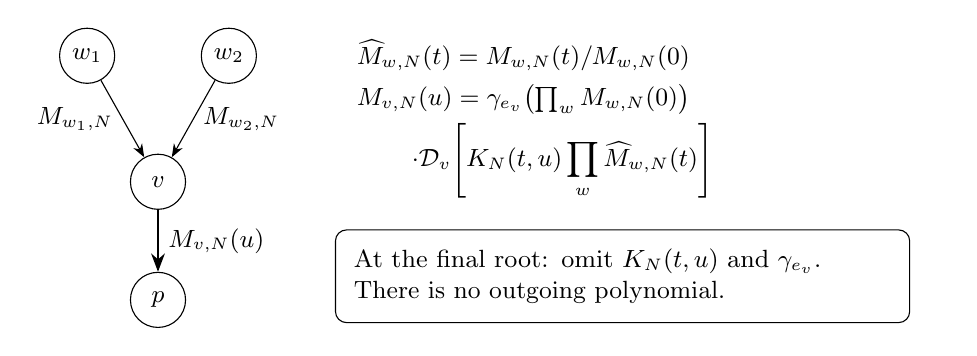
\begin{tikzpicture}[x=1cm,y=1cm,>=Stealth,vertex/.style={circle,draw,fill=white,minimum size=7mm,inner sep=1pt},every node/.style={font=\small}]
\node[vertex] (a) at (-4,1.6) {$w_1$};
\node[vertex] (b) at (-2.2,1.6) {$w_2$};
\node[vertex] (v) at (-3.1,0) {$v$};
\node[vertex] (p) at (-3.1,-1.5) {$p$};
\draw[->] (a)--node[left] {$M_{w_1,N}$} (v);
\draw[->] (b)--node[right] {$M_{w_2,N}$} (v);
\draw[->,thick] (v)--node[right] {$M_{v,N}(u)$} (p);
\node[anchor=west,align=left,text width=7.4cm] at (-.7,.8)
 {$\widehat M_{w,N}(t)=M_{w,N}(t)/M_{w,N}(0)$\\[4pt]
 $M_{v,N}(u)=\gamma_{e_v}\!\left(\prod_wM_{w,N}(0)\right)$\\[2pt]
 $\displaystyle\hspace{7mm}\cdot\mathcal D_v\!\left[K_N(t,u)\prod_w\widehat M_{w,N}(t)\right]$};
\node[draw,rounded corners,align=left,text width=6.8cm,inner sep=7pt] at (2.8,-1.2)
 {At the final root: omit $K_N(t,u)$ and $\gamma_{e_v}$. There is no outgoing polynomial.};
\end{tikzpicture}

\caption{Edges point toward the vertex whose trace is evaluated next.
The exact numbers \(M_{w,N}(0)\) are factored out before applying that
trace. The outgoing polynomial is then divided by its own exact value
at zero. Only a nonroot vertex must supply an outgoing real-decay bound;
the final root evaluates a scalar. This diagram describes contraction
order, not an isotopy of the knot.}\label{dt:recursion-figure}
\end{figure}

\section{The phase class and the variable envelopes}\label{dt:sec-4}

The inductive analytic class is

\begin{equation}\label{dt:eq-27}
h_v(0)=h'_v(0)=0,\qquad h_v(-u)=h_v(u),\qquad
 |h_v''(u)+a_0|\le a_0/20,\quad u\in\mathcal R.
\end{equation}

The leading normalized amplitude \(\alpha_v(u)/\alpha_v(0)\) is holomorphic
and nonzero on a neighborhood of the required smaller compact. Exact
subtree constants are retained:

\begin{equation}\label{dt:eq-28}
\frac{M_{v,N}(u)}{M_{v,N}(0)}
 =\frac{\alpha_v(u)}{\alpha_v(0)}e^{Nh_v(u)}(1+O(N^{-1})),
                     \quad u\in\mathcal R.
\end{equation}

As usual a slightly smaller rectangle can be used for fixed derivative
estimates; the strict margins permit an initially slightly larger one.

The global assertions attached to \(c_v\) are

\begin{equation}\label{dt:eq-29}
\left|\frac{M_{v,N}(t)}{M_{v,N}(0)}\right|
          \le CN^A e^{-Nc_v(1-\cos t)},
                         \quad t\in[-\pi,\pi],
\end{equation}

\begin{equation}\label{dt:eq-30}
\left|\frac{M_{v,N}(t+iy)}{M_{v,N}(0)}\right|
 \le CN^A e^{N[-(c_v/2)(1-\cos t)+y^2]},
                      \quad |y|\le\delta_v.
\end{equation}

For canonical representatives of degree less than \(N\), the real sup,
Chebyshev and full value-and-first-derivative norms differ by polynomial
factors, by \cite[Lemma~2.1]{Summed}. A product of degree a fixed multiple
of \(N\) is first bounded in its real sup norm and then folded in the
correct quotient; no equivalence with finite node data is asserted for
an unreduced higher-degree polynomial. In particular the reduction and
trace retain the repeated-root normals.

Here is the passage from the real bound to the strip. Write the
normalized message as a Laurent polynomial \(P(e^{\ii t})\), of powers
between \(-m\) and \(m\), where \(m<N\). The subharmonic function
\(\log|z^mP(z)|\) on the unit disk is bounded by the harmonic
function \(\log(CN^A)-Nc_v+Nc_v\Re z\). Substitute
\(z=e^{-y+\ii t}\) and divide by \(|z|^m\); for negative \(y\)
use the reciprocal polynomial. Since \(1-e^{-|y|}\le|y|\), this gives

\begin{equation}\label{dt:eq-31}
|M_{v,N}(t+iy)/M_{v,N}(0)|
 \le CN^A e^{N[-c_v(1-\cos t)+(1+c_v)|y|]}.
\end{equation}

For \(|t|\ge r_0\) use \eqref{dt:eq-3}. For \(|t|<r_0\) use the rectangle expansion and

\begin{equation}\label{dt:eq-32}
\Re h_v(t+iy)\le
       -\frac{19a_0}{40}t^2+\frac{21a_0}{40}y^2.
\end{equation}

Both arguments give \eqref{dt:eq-30}, without a conjectured quadratic estimate for
an individual high Newton basis element.

Assume the children satisfy \eqref{dt:eq-27}--\eqref{dt:eq-30}. At a nonroot vertex set

\begin{equation}\label{dt:eq-33}
A_v^{\mathrm{loc}}(t,u)=\psi(t,u)+\sum_wh_w(t),
 \quad
 C_{v,\ell}(u)=\operatorname{stat}_t
       \{A_v^{\mathrm{loc}}(t,u)+ib_vt^2/2-i\ell t\}.
\end{equation}

At the root omit \(\psi\) and \(u\). There are \(d_v\) incidences in \(t\). Hence

\begin{equation}\label{dt:eq-34}
A_v^{\mathrm{loc}}(t,u)=\psi(0,u)-a_vt^2/2+E_v(t,u),
       \quad |E_{v,tt}|,\ |E_{v,t}/t|\le a_v/20.
\end{equation}

The root constant in this formula is zero. For \(0\le\ell\le L_v=\lfloor t_0|D_v|\rfloor\)
the equation \(D_vt=-i\ell+E_{v,t}\) contracts in \(|t|\le b_0\). Indeed
\(t_0+b_0/20<b_0\). The actual solutions lie in the smaller disk
\(|t|\le t_0/(19/20)\), leaving room for the translated contours.

Writing \(E_{v,t}=tQ_v\), with \(|Q_v|\le a_v/20\), gives
\(t_{v,\ell}=-\ii\ell/(D_v-Q_v)\). Its imaginary part is
\(-\ell\Re(D_v-Q_v)/|D_v-Q_v|^2\). The numerator lies
between \(19a_v/20\) and \(21a_v/20\), and the denominator
between \((19|D_v|/20)^2\) and \((21|D_v|/20)^2\).
Therefore

\begin{equation}\label{dt:eq-35}
\frac{380}{441}\frac{\ell a_v}{|D_v|^2}
 \le-\Im t_{v,\ell}\le
 \frac{420}{361}\frac{\ell a_v}{|D_v|^2},
\end{equation}

also for complex parent \(u\). No child phase is asserted to be real on
the real axis. Its nonlinear derivative is \(t\) times a function bounded
by \(a_v/20\), so the real part of the denominator remains positive.

The normalized phase \(h_v=C_{v,1}(u)-C_{v,1}(0)\) satisfies

\begin{equation}\label{dt:eq-36}
h'_v=\psi_u(t_{v,1},u),\qquad
 h''_v=\psi_{uu}
       -\frac{\psi_{ut}^2}{A_{v,tt}^{\mathrm{loc}}+ib_v}.
\end{equation}

Using \eqref{dt:eq-17} and \(|A_{v,tt}^{\mathrm{loc}}+ib_v|\ge(19/20)|D_v|\ge(19/20)a_0\) proves \eqref{dt:eq-27},
since \(1/50+20/(19\cdot2500)<1/20\). This is uniform on the rectangle.
Charge ordering and the current-vertex drop are

\begin{equation}\label{dt:eq-37}
\Re C_{v,\ell}(u)\le\Re C_{v,1}(u)
  -\frac{190}{441}\frac{a_v}{|D_v|^2}(\ell^2-1),
 \quad
 0\le\Re\psi(0,u)-\Re C_{v,1}(u)\le\beta_v.
\end{equation}

At the root again replace \(\psi(0,u)\) by zero.

\section{Actual trace tails with the directed budgets}\label{dt:sec-5}

Divide every child by its exact nonzero value \(M_{w,N}(0)\). The induction
uses those complex constants exactly; it never estimates them by their
complete-source magnitudes. Equations \eqref{dt:eq-15} and \eqref{dt:eq-30} imply

\begin{equation}\label{dt:eq-38}
|\text{normalized trace input}(t+iy,u)|
 \le CN^A
   e^{N[\Re\psi(0,u)-A_vt^2+B_vy^2]},
                      \quad |y|\le\delta_v^{\mathrm{in}}.
\end{equation}

The root constant is zero. The factor \(2/\pi^2\) in \eqref{dt:eq-4} is exactly the
inequality \(1-\cos t\ge2t^2/\pi^2\) on the original interval.

Write \(\eta=(-1)^d\). For the actual input, an even trigonometric
polynomial of any fixed-multiple degree, the exact trace is
\begin{equation}\label{dt:trace-grid}
 \mathcal D_{n,\sigma,N}[f]
 =\frac{\eta N C_{N,n}(\sigma)}{\sin(2\pi\sigma)}
   \sum_{j=0}^{N-1}\sin\tau_j\,f(\tau_j)
                      e^{\ii nN\tau_j^2/(4\pi)},
 \quad\begin{cases}
 \tau_j=\dfrac{2\pi}{N}(d/2+\sigma-j),\\
 C_{N,n}(\sigma)=q_N^{n(d^2/4-\sigma^2/2)}.
 \end{cases}
\end{equation}
This is \cite[equation~(6.4)]{Meridian}, initially away from colliding
grids; its holomorphic limit includes every normal. To recall the exact
Fourier conversion, use
\[
 \mathcal K_\sigma(t)=
 \frac{\ii N e^{\ii Nt}}{e^{\ii Nt}-\eta e^{2\pi\ii\sigma}}
\]
on the rectangle with sides \(\pm\pi\pm\ii y_v+2\pi\sigma/N\).
The kernel has residue one at the \(N\) enclosed grid points and equals
\(\ii N e^{-Nz}/(1+e^{-Nz})\) on a vertical side
\(t=\pm\pi+\ii z+2\pi\sigma/N\). Its upper and lower horizontal
series are
\[
 -\ii N\sum_{\ell\ge1}\eta^\ell
       e^{-2\pi\ii\ell\sigma}e^{\ii\ell Nt},\qquad
 \ii N\left(1+\sum_{\ell\ge1}\eta^\ell
       e^{2\pi\ii\ell\sigma}e^{-\ii\ell Nt}\right).
\]
Move each entire term to a fixed horizontal segment, retaining its short
endpoint connectors. Reflect the upper integral by \(t\mapsto-t\),
with the boundary orientation; \(\sin t\,f(t)e^{\ii nNt^2/(4\pi)}\)
is odd. The paired coefficients are therefore
\begin{equation}\label{dt:eq-39}
 c_{\ell,N}(\sigma)=\eta^{\ell-1}
 U_{\ell-1}(\cos2\pi\sigma),\qquad c_{1,N}=1,
\end{equation}
with common prefactor \(-N^2C_{N,n}/(\pi\ii)\).
The zero-mode integral on the real interval vanishes by oddness, but its
endpoint currents remain. These algebraic steps are also written in
\cite[Section~6.1]{Summed}; they impose no condition on the twists or
sum over vertices. In particular there is no later sum of unexamined
equal-action signs.

For \(\ell>L_v\), moving the single-grid rectangle by \(y_v\) costs, after
maximizing the chirp term in the real variable, at most \(C_v y_v^2\).
Since \(\ell>L_v\) implies \(\ell>t_0|D_v|\), \eqref{dt:eq-6} gives a tail loss at least

\begin{equation}\label{dt:eq-40}
t_0|D_v|y_v-C_vy_v^2\ge\frac12t_0|D_v|y_v.
\end{equation}

Successive charges have the additional factor \(\exp(-Ny_v)\). The exact
fixed-compact growth of \eqref{dt:eq-39} is absorbed for all sufficiently large N.
This starting level may depend on the fixed vertex.

At an original endpoint \(\pm\pi\), the chirp and finite-charge connectors cost
at most

\begin{equation}\label{dt:eq-41}
(\pi|b_v|+t_0|D_v|)y_v+B_vy_v^2
                            \le A_v\pi^2/4.
\end{equation}

Thus their loss is at least \(A_v\pi^2/2\). This includes the original
zero-mode current. Nothing is inferred by dropping the endpoint terms
of the nonperiodic chirp.

For a retained charge, restrict its real integral to \([-r_0,r_0]\).
Its complement loses \(A_vr_0^2\) by \eqref{dt:eq-38}. Translate the retained interval
to \(\Im t_{v,\ell}\). Its endpoints remain in the analytic rectangle. The
original local Young inequality, now on this larger real interval,
is

\begin{equation}\label{dt:eq-42}
\begin{aligned}
 \Re\{A_v^{\mathrm{loc}}(t-iz,u)+ib_v(t-iz)^2/2-i\ell(t-iz)\}
 &\le\Re\psi(0,u)-a_vt^2/8\\
 &\quad+\left[\frac{21}{40}a_v+
                 \frac{2b_v^2}{(14/5)a_v}\right]z^2-\ell z.
\end{aligned}
\end{equation}

For \(0\le z\le-\Im t_{v,\ell}\), the last line after its quadratic term is
at most \(-\ell z/8\), since \((420/361)\max(21/40,5/7)=300/361<7/8\).
Every such connector therefore loses at least \(a_vr_0^2/8\).
The translated horizontal saddle has negative real quadratic part
at most \(-(19/20)a_v\). The physical sine factor is nonzero at \(t_{v,\ell}\).

Equations \eqref{dt:eq-40}--\eqref{dt:eq-42} give an error of at most
\(CN^A\exp N[\Re\psi(0,u)-\eta_v]\). Nonminimal charges are their saddle
terms plus this absolute error; no relative approximation is asserted
at a much lower nonminimal action. Conditions \eqref{dt:eq-8} and \eqref{dt:eq-37} put the
whole conditional error strictly below the first charge. Equation
\eqref{dt:eq-39} gives its nonzero coefficient for both parities. This establishes
\eqref{dt:eq-28} and nonvanishing of the exact \(M_{v,N}(0)\).

For the child inputs, their exact analytic logarithms differ from the
limiting phases by \(O(N^{-1})\), with fixed derivatives on the required
smaller compact. The finite product of those corrections is retained
in the amplitude, or moves the saddle by \(O(N^{-1})\). As the tree is fixed,
it spends no new exponential budget. The leading amplitude is a product
of nonzero edge, child and Gaussian factors. All N-dependent physical
crossing and carrier phases remain in \(M_{v,N}(0)\); its normalized leading
amplitude does not conceal such phases.

The full physical trace and the first-charge approximation are
holomorphic in the formal meridian variables. As in the original
proof, first take parameter circles avoiding collisions and then apply
the maximum principle to their whole difference. This covers every
actual \(\sigma_v=0,\pm s\), including normal limits. No isolated divided
current is declared removable without its companions.

\section{Regenerating the outgoing real bound}\label{dt:sec-6}

Lemma~2.1 of \cite{Summed} compares the real sup norm, the
Chebyshev norm, and the complete value-and-first-derivative norm by
polynomial factors. It also bounds the physical fixed-power crossing
and the full quotient trace. These estimates apply to polynomial
products of degree a fixed multiple of \(N\); that multiple can depend
on the degree of this fixed vertex. For real \(u\), \eqref{dt:eq-14},
the polynomial real sup bounds of the normalized children, the actual
fixed-power crossing polynomial, Chebyshev folding in the correct
quotient, and the full top-coefficient functional give

\begin{equation}\label{dt:eq-43}
|M_{v,N}(u)|\le CN^A
       \left|\prod_wM_{w,N}(0)\right|
                  e^{N[2G_0-k_0(1-\cos u)]}.
\end{equation}

This retains repeated-root derivatives and all fixed normals. Dividing
by the nonzero first-charge value at zero costs at most \(\beta_v\). For
\(|u|\ge r_0\), \eqref{dt:eq-9} absorbs that cost and yields \eqref{dt:eq-29}. For \(|u|<r_0\), \eqref{dt:eq-28}
and \eqref{dt:eq-32} give the stronger estimate, since \(c_v<k_0\ll19a_0/20\).
Equation \eqref{dt:eq-30} follows by Section~\ref{dt:sec-4}. Thus the induction closes with
the selected directed budgets, rather than a common decay constant.

There is no outgoing real bound at the final root. Imposing \eqref{dt:eq-9} there
would be an unnecessary restriction. Its only normalization comparison
is the conditional trace estimate \eqref{dt:eq-8}.

\section{Original action, geometry, and scope}\label{dt:sec-7}

Restore the exact subtree constants successively. Stationary
elimination in \eqref{dt:eq-33} gives the original joint equations

\begin{equation}\label{dt:eq-44}
\sum_{e\sim v}\psi_{e,\tau_v}
                      +\frac{in_v\tau_v}{2\pi}=i.
\end{equation}

The exact child constants telescope to the original critical value

\begin{equation}\label{dt:eq-45}
\mathcal C(\mathbf1)=\operatorname{stat}_{\boldsymbol\tau}
 \left[\sum_e\psi_e+
       \frac{i}{4\pi}\sum_vn_v\tau_v^2-i\sum_v\tau_v\right].
\end{equation}

Back-substitute from the final root: its first-charge angle belongs to
the rectangle, so each child's selected parent value does also, and
the same statement continues down the finite tree. Every restored angle
has modulus at most \(1/[(19/20)|D_v|]\). Thus the vector satisfying
\eqref{dt:eq-44} lies inside the full simultaneous small-angular uniqueness
polydisk, not just the conditional disks used during elimination.
The existing contraction identifies it with the same branch as the
marked positive charge path of \cite[Theorem~1.1]{Geometry}. In fact
\(20/(19|D_v|)<10^{-2}\). Indeed
\eqref{dt:eq-8} implies

\begin{equation}\label{dt:eq-46}
\sqrt{d_v^2+n_v^2}=2\pi|D_v|\ge 2\pi\,2^{15}>630.
\end{equation}

\cite[Theorem~1.1]{Geometry} applies with no sum condition.
The edge functions agree: their derivatives are \eqref{dt:psi} and
their complete values satisfy \(2G_0=v_{\rm oct}/\pi\), as in
\cite[Section~7]{Summed}. Write \(n_v=\epsilon_v-2p_v\), with
\(\epsilon_v\in\{-1,0,1\}\), in the original disk frame. The
primitive periods supplied by the geometric theorem are
\[
 U_v=-2\pi\Psi_{\tau_v}-\ii\epsilon_v\tau_v,
 \qquad V_v=2\ii\tau_v.
\]
Equation \eqref{dt:eq-44} therefore gives the full continued relation
\(U_v+p_vV_v=-2\pi\ii\). The imported theorem proves its primitive
winding, smooth metric completion, and complete main cusp; we do not
infer these facts from an exponentiated equation.
Its original ordered two-octahedron cut, odd seam and calibrated action identify \(2\pi\Re\mathcal C(\mathbf1)\) with the volume of the actual
filled knot complement. This is a geometric input, not a deduction
from the quantum saddle alone.

There are \(|E|\) edge Gaussians \(N^{-3/2}\) and \(|V|\) trace Gaussians \(N^{3/2}\);
\(|V|=|E|+1\) leaves the original \(N^{3/2}\) power with nonzero amplitude.
The exact first Fourier coefficient is one. The retained edge insertion
has leading value one, and the scalar ledger remains precisely \eqref{dt:scalars}.
At \(s=0\), all edge gammas and paired insertions equal one.
The exact outside scalar is
\[
 \Omega_N=\theta_d^{-w(D)}\prod_vC_{N,n_v}(0)
       =q_N^{d^2(2w(D)+\sum_v n_v)/4},
 \qquad \theta_d=q_N^{-d^2/2}.
\]
The remaining leading coefficient is independent of \(N\), nonzero,
and the same through both parities. This proves the full leading
asymptotic in Theorem~\ref{dt:main}.
For bounded \(s\), the first-charge coefficient is still one, the
paired insertion has leading value one, and all normalized leading
amplitudes are unchanged. Restoring the exact scalar ledger of
\cite[Proposition~8.1]{Meridian} gives \(A_N(s)H_N(s)\).
The finite product of relative \(1+O_R(N^{-1})\) factors proves
\eqref{dt:profile}. Its nonvanishing follows uniformly on every
fixed disk \(R<1\), since \(A_N\) and \(H_N\) have no zeros there.
Together with the geometric identification above this proves
Theorem~\ref{dt:main}.

The criterion allows different strip and real-decay budgets and a
different choice of final vertex. It is not the assertion that arbitrary
capped short-twist islands can be substituted as black-box messages.
Such an island requires a multi-boundary version of the conditional
normalization proved here for an actual edge. The pointwise source
estimates on the older tiny disk alone do not supply that extension.

\section{Uniform local consequences and concrete constructions}\label{dt:sec-8}

The directed criterion has the following simple consequence:

\begin{equation}\label{dt:eq-47}
|n_v|\ge2^{27}\quad\text{at every vertex}
             \quad\Longrightarrow\quad\text{Theorem~\ref{dt:main}}.
\end{equation}

This sufficient constant is independent of the number of vertices,
their degrees and the choice of root. Here is a proof covering all
degrees simultaneously. Choose \(c_v=k_0/2\) at every nonroot vertex
and write \(\delta\) for their common value in \eqref{dt:eq-3}. The elementary
cosine estimate gives

\begin{equation}\label{dt:eq-48}
\chi\ge\frac{r_0^2}{2}-\frac{r_0^4}{24}
       =2^{-9}\frac{3071}{3072}>2^{-10},\qquad
                          \delta>2^{-30}.
\end{equation}

At any vertex, including the root, put
\(\mathcal R_v=\sqrt{d_v^2+n_v^2}\). Then

\begin{equation}\label{dt:eq-49}
A_v\ge\frac{k_0d_v}{2\pi^2},\qquad B_v\le16d_v,
 \qquad C_v\le\frac{\mathcal R_v^2}{8k_0d_v}.
\end{equation}

For the last inequality use \(16\le1/(8k_0)\). Each of the four
branches of the minimum in \eqref{dt:eq-6} consequently has the following lower
bound, respectively:

\begin{equation}\label{dt:eq-50}
\frac\delta2,\qquad
 \frac{t_0k_0d_v}{\pi\mathcal R_v},\qquad
 \frac{k_0d_v}{16\mathcal R_v},\qquad 2^{-12}.
\end{equation}

The second displayed quantity is smaller than the third and fourth.
For the third bound, use
\(\pi|b_v|+t_0|D_v|\le\mathcal R_v(1+t_0/\pi)/2\).
Thus every branch of \eqref{dt:eq-7}, not just its tail branch, is bounded below by

\begin{equation}\label{dt:eq-51}
\eta_v\ge\min\left\{
       \frac{t_0\mathcal R_v\delta}{8\pi},
       \frac{t_0^2 k_0d_v}{4\pi^2}\right\}.
\end{equation}

Indeed the second entry here is smaller than each of the other three
entries in \eqref{dt:eq-7}, by their explicit values and \(t_0\ll r_0\).
On the other hand

\begin{equation}\label{dt:eq-52}
\beta_v=\frac{420\pi}{361}\frac{d_v}{\mathcal R_v^2}
                       <\frac{4d_v}{\mathcal R_v^2}.
\end{equation}

For comparison with half the first entry of \eqref{dt:eq-51}, it suffices that
\(\mathcal R_v^2>64\pi/(t_0\delta)\), since \(d_v\le\mathcal R_v\).
The right side is less than \(2^{52}\), using \(\pi<4\) and \eqref{dt:eq-48}.
For comparison with half the second entry it suffices that
\(\mathcal R_v^2>32\pi^2/(t_0^2k_0)\), whose right side is less
than \(2^{53}\), since \(\pi^2<10\). Both inequalities follow
strictly from \(\mathcal R_v^2\ge n_v^2\ge2^{54}\).
The charge-cut condition in \eqref{dt:eq-8} follows as well.

For the outgoing patch, the sharper elementary estimate is

\begin{equation}\label{dt:eq-53}
\beta_v\le\frac{210\pi}{361|n_v|}
 \le\frac{330}{361}\,2^{-26}
 <\frac{3071}{3072}\,2^{-26}
 \le\frac{k_0}2\chi.
\end{equation}

Here \(\pi<22/7\),
\(d_v/(d_v^2+n_v^2)\le1/(2|n_v|)\), and the displayed rational
comparison prove \eqref{dt:eq-9} for every degree. This completes the corollary
without a numerical scan or a threshold depending on the tree.

The same proof gives a mixed condition, chosen independently at each
vertex:

\begin{equation}\label{dt:eq-53a}
\boxed{\qquad
       d_v\ge2^{28}\quad\text{or}\quad |n_v|\ge2^{27}
               \qquad\text{for every }v.\qquad}
\end{equation}

Under the degree alternative, \(\mathcal R_v^2\ge d_v^2\ge2^{56}\)
proves the same two tail comparisons, while

\begin{equation}\label{dt:eq-53b}
\beta_v\le\frac{420\pi}{361d_v}
             \le\frac{330}{361}\,2^{-26}
                    <\frac{k_0}2\chi
\end{equation}

is the same outgoing patch bound. Neither alternative needs to hold
uniformly over all vertices. In particular, the high-degree vertices
may retain any fixed signed powers, including zero and small nonzero
powers. No sum over the number of such vertices occurs.

Here is a precise extension construction illustrating that freedom.
Start with any fixed ordered circle-tree core whose original endpoint
pairing closes to a knot and has no internal closed component. Retain
all its fixed signed powers. At every core vertex choose one of its
actual product slots next to its crossing box and insert a consecutive
stack of an even number \(B\ge2^{28}\) of new terminal pieces. Every
new leaf has a fixed odd power satisfying

\begin{equation}\label{dt:eq-53c}
|n_{\mathrm{leaf}}|\ge2^{27}+1.
\end{equation}

The physical quarter-turn of an odd two-strand braid has diagonal
pairing \(X=\{02,13\}\); this pairing is invariant under the
quarter-turn. An even ordered stack of these leaves has the through
pairing \(I=\{03,12\}\) and creates no internal circle. Inserting it
in the specified slot therefore preserves the original local endpoint
pairing in that actual frame. This is a pairing calculation, not an
isotopy removing the new tangles. At the original closing box the same
insertion takes place inside its local ball. An added terminal leaf may
then be chosen as the recursive root using the original closed-collar
move with its induced frame reversal and factor order retained.

Thus the resulting diagram is again a knot, while its knot type may
change. Each old vertex now satisfies the degree alternative and each
new leaf satisfies the twist alternative in \eqref{dt:eq-53a}. The resulting actual
knot complement is hyperbolic and satisfies Theorem~\ref{dt:main}. The number and
arrangement of prescribed short-power vertices are arbitrary but fixed;
the number \(B\) does not depend on their total count.

\begin{figure}[t]
\centering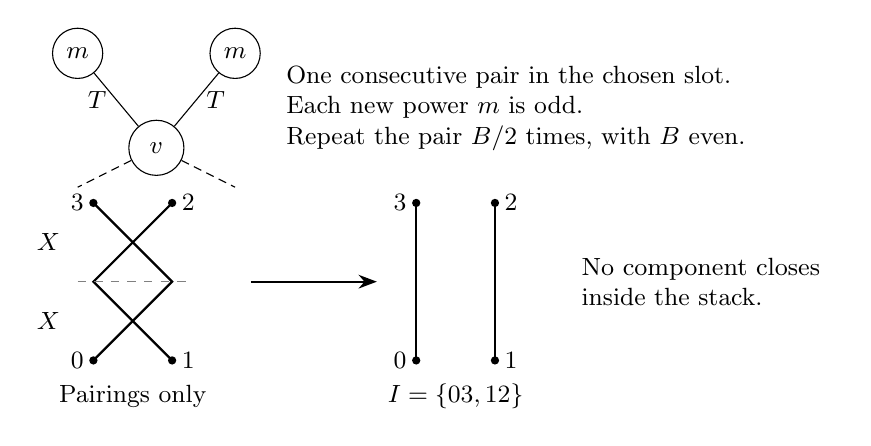
\begin{tikzpicture}[x=1cm,y=1cm,>=Stealth,every node/.style={font=\small}]
\node[circle,draw,minimum size=7mm] (v) at (-3,1.5) {$v$};
\node[circle,draw,minimum size=6mm] (l) at (-4,2.7) {$m$};
\node[circle,draw,minimum size=6mm] (r) at (-2,2.7) {$m$};
\draw (v)--node[left] {$T$}(l);
\draw (v)--node[right] {$T$}(r);
\draw[densely dashed] (v)--(-4,1);
\draw[densely dashed] (v)--(-2,1);
\node[align=left,text width=6.7cm] at (2,2)
 {One consecutive pair in the chosen slot.\\Each new power $m$ is odd.\\Repeat the pair $B/2$ times, with $B$ even.};
\begin{scope}[shift={(-3.8,-1.2)}]
\draw[thick] (0,0)--(1,1)--(0,2);
\draw[thick] (1,0)--(0,1)--(1,2);
\draw[dashed,gray] (-.2,1)--(1.2,1);
\foreach \x/\y in {0/0,1/0,0/2,1/2}{\fill (\x,\y) circle(1.5pt);}
\node[left] at (0,0) {$0$};\node[right] at (1,0) {$1$};
\node[right] at (1,2) {$2$};\node[left] at (0,2) {$3$};
\node[left] at (-.3,.5) {$X$};\node[left] at (-.3,1.5) {$X$};
\node at (.5,-.45) {Pairings only};
\end{scope}
\draw[->,thick] (-1.8,-.2)--(-.2,-.2);
\begin{scope}[shift={(.3,-1.2)}]
\draw[thick] (0,0)--(0,2);\draw[thick] (1,0)--(1,2);
\foreach \x/\y in {0/0,1/0,0/2,1/2}{\fill (\x,\y) circle(1.5pt);}
\node[left] at (0,0) {$0$};\node[right] at (1,0) {$1$};
\node[right] at (1,2) {$2$};\node[left] at (0,2) {$3$};
\node at (.5,-.45) {$I=\{03,12\}$};
\end{scope}
\node[align=left,text width=3.2cm] at (4,-.2) {No component closes inside the stack.};
\end{tikzpicture}

\caption{The upper drawing records tangle operations, not a knot
projection. In the construction, each drawn pair represents \(B/2\)
consecutive pairs inserted in one chosen product slot. The lower
pairing calculation is \(X\circ X=I\), with no internal component;
it preserves the original closure's component count, not its knot type.}
\label{dt:leaves-figure}
\end{figure}

The earlier uniform local condition is also a corollary:
\begin{corollary}\label{dt:local}
If \(\max_v d_v/(d_v^2+n_v^2)\le2^{-120}\), then the conclusions
of Theorem~\ref{dt:main} hold.
\end{corollary}
\begin{proof}
If both \(d_v<2^{28}\) and \(|n_v|<2^{27}\), then
\(d_v^2+n_v^2<2^{57}\). Since \(d_v\ge1\), this would give
\(d_v/(d_v^2+n_v^2)>2^{-57}>2^{-120}\). Thus every vertex
satisfies \eqref{dt:eq-53a}. This proof uses the directed theorem,
not a summability hypothesis over vertices.
\end{proof}

\section{A star beyond both previous quantitative tests}\label{dt:sec-9}

Consider an ordered star rooted at its central vertex, of odd degree
\(d=30{,}000{,}001\). Set its power to 2 and every terminal power to the fixed
odd integer \(2^{60}+1\). Choose \(c_v=k_0/2\) on every leaf.

The knot pairing can be checked in the original terminal-root syntax,
even though the finite contraction is evaluated from the center. Label
the boundary points lower left, lower right, upper right, upper left
by \(0,1,2,3\). The even and odd braid pairings are respectively

\begin{equation}\label{dt:eq-54a}
I=\{03,12\},\qquad X=\{02,13\};\qquad
 T(I)=H=\{01,23\},\quad T(X)=X.
\end{equation}

At a terminal root there are \(d-1\) other leaves. Their turned odd
braids have pairing \(X\); their ordered product has pairing \(I\)
because \(d-1\) is even. The central power \(2\) preserves it. Its
actual quarter-turn has pairing \(H\), and stacking the root's odd
braid against \(H\) still gives \(H\), with no internal closed arc.
Cylindrical closure joins \(03\) and \(12\), so it closes \(H\)
into one component. All intermediate products before that last stack
are two through-strand braids. There is no hidden internal component.

The criterion can be verified by rational enclosures without expanding this large
tree. All leaves have the same data. The center has approximately

\begin{equation}\label{dt:eq-54}
\beta_o=1.219\,10^{-7},\qquad
 \eta_o=2.713\,10^{-7},\qquad
       \frac{\beta_o}{\eta_o/2}<0.9.
\end{equation}

Every leaf has a much smaller ratio. The root does not satisfy the
nonroot patch inequality for any \(c>0\), because \(\beta_o>k_0\chi\).
Nevertheless its exact final trace satisfies \eqref{dt:eq-8}. Thus that outgoing
patch must not be charged to a root that sends no message.

Moreover

\begin{equation}\label{dt:eq-55}
\sum_v\frac{d_v}{d_v^2+n_v^2}
       >\frac{30,000,001}{30,000,001^2+4}>2^{-25},
\end{equation}

and its maximum is far above \(2^{-120}\). The example therefore lies beyond
both published quantitative alternatives. Its size and all its powers
are fixed; it is not an N-growing family. The constant sizes are coarse,
and no optimality assertion is intended.

Here are rational enclosures proving the inequalities rather than
inferring them from those decimal values. Put

\begin{equation}\label{dt:eq-56}
\pi_- =3,\quad \pi_+=22/7,\quad c=k_0/2,\quad
 \chi_-=r_0^2/2-r_0^4/24,\quad
 \delta_- =\frac{c\chi_-}{4(1+c)}.
\end{equation}

At the central vertex use the conservative height
\(y_* =\delta_-/2\). It is at most each branch of \eqref{dt:eq-6}. For example,
with

\begin{equation}\label{dt:eq-57}
D_- =\frac d{2\pi_+},\quad D_+=\frac{d+1}{2\pi_-},\quad
 A_- =\frac{dc}{\pi_+^2},\quad
 C_+=d+\frac{\pi_-^{-2}}{4A_-},
\end{equation}

the three non-strip comparisons are

\begin{equation}\label{dt:eq-58}
y_*<\frac{t_0D_-}{4C_+},\qquad
 y_*<\frac{dc}{8(1+t_0D_+)},\qquad y_*^2<\frac c8.
\end{equation}

The strip comparison follows from \(\delta\ge\delta_-\).
Every quantity in \eqref{dt:eq-56}--\eqref{dt:eq-58} is rational. Direct cross-multiplication
also gives

\begin{equation}\label{dt:eq-59}
\frac{2[420\pi_+d/(361(d^2+4))]}
             {t_0D_-y_*/2}<\frac9{10},
 \qquad
 2\frac{420\pi_+d}{361(d^2+4)}
 <\min\left\{\frac{dc}{2},\ A_-r_0^2,
                          \frac{D_-r_0^2}{8}\right\}.
\end{equation}

These compare the upper bound for twice the first-charge drop with
all four lower bounds for \(\eta_o\). The charge cutoff is greater
than two.

For a leaf with \(n=2^{60}+1\), take
\(y_*=t_0k_0/(2n)\). The same direct rational comparisons, using
\(D_-=n/(2\pi_+)\), \(D_+=(n+1)/(2\pi_-)\),
\(A_-=2k_0/\pi_+^2\), and
\(C_+=16+[n/(2\pi_-)]^2/(4A_-)\), put this height below each
branch of \eqref{dt:eq-6}. They give a lower bound greater than \(2^{-49}\)
for every entry of \eqref{dt:eq-7}, while \(\beta_v<2^{-117}\).
The outgoing patch follows from
\(\beta_v<(k_0/2)\chi_-\). This proves the leaf inequalities.


\section{Finite reproduction and limitations}\label{dt:reproduction}
From the repository root run
\begin{verbatim}
python3 papers/directed-tree-asymptotics/check.py \\
    --output /tmp/directed-tree-check.json
\end{verbatim}
The record pins its source files. It reuses the exact rational budget
and endpoint-pairing calculations, and the finite comparison of quotient
messages with full root-grid and first-normal contractions. The examples
in that comparison use formal independent vertex parameters; this tests
the finite algebra, not the existence of additional diagrams.
The checker also verifies the elementary implication from the older
local condition and includes negative controls for a lost root
exemption and an odd rather than even inserted stack. Finite checks
neither prove the uniform analytic induction nor replace the imported
geometric theorem.

\begin{thebibliography}{9}
\bibitem{Meridian}
\emph{Exact Newton calculus for tangles with a moving meridian},
companion paper, Propositions~6.1 and~8.1, Theorem~7.1.
\url{https://sashakolpakov.github.io/murakamis_dream/papers/meridian-tangles.pdf}.
\bibitem{Summed}
\emph{Degree and twist estimates for circle-tree invariants},
companion paper, Lemma~2.1 and Sections~3, 4 and~6.1.
\url{https://sashakolpakov.github.io/murakamis_dream/papers/circle-tree-asymptotics.pdf}.
\bibitem{Factorial}
\emph{Holomorphic source asymptotics and volume limits for Conway closures},
companion paper, Lemma~2.1.
\url{https://sashakolpakov.github.io/murakamis_dream/papers/conway-asymptotics.pdf}.
\bibitem{Geometry}
\emph{Positive octahedra and primitive fillings for trees of crossing circles}, companion paper, Theorem~1.1.
\url{https://sashakolpakov.github.io/murakamis_dream/papers/circle-tree-geometry.pdf}.
\end{thebibliography}
\end{document}
